\documentclass[tikz,border=4pt]{standalone}
\usepackage{helvet}
\renewcommand{\familydefault}{\sfdefault}
\definecolor{talnGreen}{HTML}{2F7D4A}
\definecolor{widthOne}{HTML}{3973AC}
\definecolor{widthTwo}{HTML}{D07A28}
\definecolor{widthThree}{HTML}{B44949}
\begin{document}
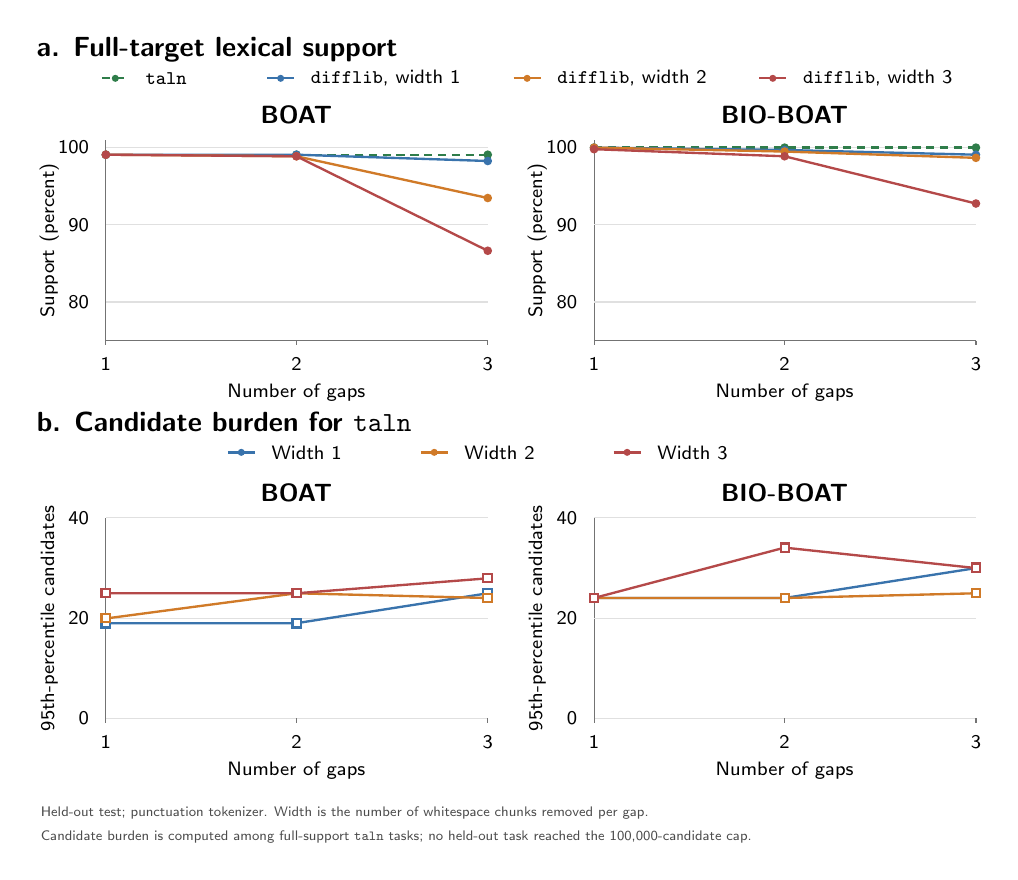
\begin{tikzpicture}[x=1cm,y=1cm]
\node[anchor=west,font=\bfseries] at (0.00,10.15) {a. Full-target lexical support};
\draw[densely dashed,color=talnGreen,line width=0.85pt] (0.95,9.78) -- (1.29,9.78);
\fill[talnGreen] (1.12,9.78) circle (0.045);
\node[anchor=west,font=\scriptsize] at (1.38,9.78) {\texttt{taln}};
\draw[color=widthOne,line width=0.85pt] (3.05,9.78) -- (3.39,9.78);
\fill[widthOne] (3.22,9.78) circle (0.045);
\node[anchor=west,font=\scriptsize] at (3.48,9.78) {\texttt{difflib}, width 1};
\draw[color=widthTwo,line width=0.85pt] (6.18,9.78) -- (6.52,9.78);
\fill[widthTwo] (6.35,9.78) circle (0.045);
\node[anchor=west,font=\scriptsize] at (6.61,9.78) {\texttt{difflib}, width 2};
\draw[color=widthThree,line width=0.85pt] (9.30,9.78) -- (9.64,9.78);
\fill[widthThree] (9.47,9.78) circle (0.045);
\node[anchor=west,font=\scriptsize] at (9.73,9.78) {\texttt{difflib}, width 3};
\node[font=\small\bfseries] at (3.42,9.32) {BOAT};
\draw[black!55] (1.00,6.45) -- (5.85,6.45);
\draw[black!55] (1.00,6.45) -- (1.00,9.00);
\draw[black!12] (1.00,6.94) -- (5.85,6.94);
\node[anchor=east,font=\scriptsize] at (0.91,6.94) {80};
\draw[black!12] (1.00,7.92) -- (5.85,7.92);
\node[anchor=east,font=\scriptsize] at (0.91,7.92) {90};
\draw[black!12] (1.00,8.90) -- (5.85,8.90);
\node[anchor=east,font=\scriptsize] at (0.91,8.90) {100};
\draw[black!55] (1.00,6.45) -- (1.00,6.39);
\node[anchor=north,font=\scriptsize] at (1.00,6.35) {1};
\draw[black!55] (3.42,6.45) -- (3.42,6.39);
\node[anchor=north,font=\scriptsize] at (3.42,6.35) {2};
\draw[black!55] (5.85,6.45) -- (5.85,6.39);
\node[anchor=north,font=\scriptsize] at (5.85,6.35) {3};
\node[anchor=north,font=\scriptsize] at (3.42,6.02) {Number of gaps};
\node[rotate=90,font=\scriptsize] at (0.28,7.72) {Support (percent)};
\draw[densely dashed,color=talnGreen,line width=0.85pt] (1.00,8.81) -- (3.42,8.81) -- (5.85,8.81);
\fill[talnGreen] (1.00,8.81) circle (0.055);
\fill[talnGreen] (3.42,8.81) circle (0.055);
\fill[talnGreen] (5.85,8.81) circle (0.055);
\draw[color=widthOne,line width=0.85pt] (1.00,8.81) -- (3.42,8.81) -- (5.85,8.73);
\fill[widthOne] (1.00,8.81) circle (0.055);
\fill[widthOne] (3.42,8.81) circle (0.055);
\fill[widthOne] (5.85,8.73) circle (0.055);
\draw[color=widthTwo,line width=0.85pt] (1.00,8.81) -- (3.42,8.79) -- (5.85,8.26);
\fill[widthTwo] (1.00,8.81) circle (0.055);
\fill[widthTwo] (3.42,8.79) circle (0.055);
\fill[widthTwo] (5.85,8.26) circle (0.055);
\draw[color=widthThree,line width=0.85pt] (1.00,8.81) -- (3.42,8.79) -- (5.85,7.59);
\fill[widthThree] (1.00,8.81) circle (0.055);
\fill[widthThree] (3.42,8.79) circle (0.055);
\fill[widthThree] (5.85,7.59) circle (0.055);
\node[font=\small\bfseries] at (9.62,9.32) {BIO-BOAT};
\draw[black!55] (7.20,6.45) -- (12.05,6.45);
\draw[black!55] (7.20,6.45) -- (7.20,9.00);
\draw[black!12] (7.20,6.94) -- (12.05,6.94);
\node[anchor=east,font=\scriptsize] at (7.11,6.94) {80};
\draw[black!12] (7.20,7.92) -- (12.05,7.92);
\node[anchor=east,font=\scriptsize] at (7.11,7.92) {90};
\draw[black!12] (7.20,8.90) -- (12.05,8.90);
\node[anchor=east,font=\scriptsize] at (7.11,8.90) {100};
\draw[black!55] (7.20,6.45) -- (7.20,6.39);
\node[anchor=north,font=\scriptsize] at (7.20,6.35) {1};
\draw[black!55] (9.62,6.45) -- (9.62,6.39);
\node[anchor=north,font=\scriptsize] at (9.62,6.35) {2};
\draw[black!55] (12.05,6.45) -- (12.05,6.39);
\node[anchor=north,font=\scriptsize] at (12.05,6.35) {3};
\node[anchor=north,font=\scriptsize] at (9.62,6.02) {Number of gaps};
\node[rotate=90,font=\scriptsize] at (6.48,7.72) {Support (percent)};
\draw[densely dashed,color=talnGreen,line width=0.85pt] (7.20,8.90) -- (9.62,8.90) -- (12.05,8.90);
\fill[talnGreen] (7.20,8.90) circle (0.055);
\fill[talnGreen] (9.62,8.90) circle (0.055);
\fill[talnGreen] (12.05,8.90) circle (0.055);
\draw[color=widthOne,line width=0.85pt] (7.20,8.90) -- (9.62,8.87) -- (12.05,8.81);
\fill[widthOne] (7.20,8.90) circle (0.055);
\fill[widthOne] (9.62,8.87) circle (0.055);
\fill[widthOne] (12.05,8.81) circle (0.055);
\draw[color=widthTwo,line width=0.85pt] (7.20,8.90) -- (9.62,8.85) -- (12.05,8.77);
\fill[widthTwo] (7.20,8.90) circle (0.055);
\fill[widthTwo] (9.62,8.85) circle (0.055);
\fill[widthTwo] (12.05,8.77) circle (0.055);
\draw[color=widthThree,line width=0.85pt] (7.20,8.88) -- (9.62,8.79) -- (12.05,8.19);
\fill[widthThree] (7.20,8.88) circle (0.055);
\fill[widthThree] (9.62,8.79) circle (0.055);
\fill[widthThree] (12.05,8.19) circle (0.055);
\node[anchor=west,font=\bfseries] at (0.00,5.42) {b. Candidate burden for \texttt{taln}};
\draw[color=widthOne,line width=0.85pt] (2.55,5.03) -- (2.89,5.03);
\fill[widthOne] (2.72,5.03) circle (0.045);
\node[anchor=west,font=\scriptsize] at (2.98,5.03) {Width 1};
\draw[color=widthTwo,line width=0.85pt] (5.00,5.03) -- (5.34,5.03);
\fill[widthTwo] (5.17,5.03) circle (0.045);
\node[anchor=west,font=\scriptsize] at (5.43,5.03) {Width 2};
\draw[color=widthThree,line width=0.85pt] (7.45,5.03) -- (7.79,5.03);
\fill[widthThree] (7.62,5.03) circle (0.045);
\node[anchor=west,font=\scriptsize] at (7.88,5.03) {Width 3};
\node[font=\small\bfseries] at (3.42,4.52) {BOAT};
\draw[black!55] (1.00,1.65) -- (5.85,1.65);
\draw[black!55] (1.00,1.65) -- (1.00,4.20);
\draw[black!12] (1.00,1.65) -- (5.85,1.65);
\node[anchor=east,font=\scriptsize] at (0.91,1.65) {0};
\draw[black!12] (1.00,2.92) -- (5.85,2.92);
\node[anchor=east,font=\scriptsize] at (0.91,2.92) {20};
\draw[black!12] (1.00,4.20) -- (5.85,4.20);
\node[anchor=east,font=\scriptsize] at (0.91,4.20) {40};
\draw[black!55] (1.00,1.65) -- (1.00,1.59);
\node[anchor=north,font=\scriptsize] at (1.00,1.55) {1};
\draw[black!55] (3.42,1.65) -- (3.42,1.59);
\node[anchor=north,font=\scriptsize] at (3.42,1.55) {2};
\draw[black!55] (5.85,1.65) -- (5.85,1.59);
\node[anchor=north,font=\scriptsize] at (5.85,1.55) {3};
\node[anchor=north,font=\scriptsize] at (3.42,1.22) {Number of gaps};
\node[rotate=90,font=\scriptsize] at (0.28,2.92) {95th-percentile candidates};
\draw[color=widthOne,line width=0.85pt] (1.00,2.86) -- (3.42,2.86) -- (5.85,3.24);
\filldraw[fill=white,draw=widthOne,line width=0.75pt] (0.945,2.806) rectangle (1.055,2.916);
\filldraw[fill=white,draw=widthOne,line width=0.75pt] (3.370,2.806) rectangle (3.480,2.916);
\filldraw[fill=white,draw=widthOne,line width=0.75pt] (5.795,3.189) rectangle (5.905,3.299);
\draw[color=widthTwo,line width=0.85pt] (1.00,2.92) -- (3.42,3.24) -- (5.85,3.18);
\filldraw[fill=white,draw=widthTwo,line width=0.75pt] (0.945,2.870) rectangle (1.055,2.980);
\filldraw[fill=white,draw=widthTwo,line width=0.75pt] (3.370,3.189) rectangle (3.480,3.299);
\filldraw[fill=white,draw=widthTwo,line width=0.75pt] (5.795,3.125) rectangle (5.905,3.235);
\draw[color=widthThree,line width=0.85pt] (1.00,3.24) -- (3.42,3.24) -- (5.85,3.43);
\filldraw[fill=white,draw=widthThree,line width=0.75pt] (0.945,3.189) rectangle (1.055,3.299);
\filldraw[fill=white,draw=widthThree,line width=0.75pt] (3.370,3.189) rectangle (3.480,3.299);
\filldraw[fill=white,draw=widthThree,line width=0.75pt] (5.795,3.380) rectangle (5.905,3.490);
\node[font=\small\bfseries] at (9.62,4.52) {BIO-BOAT};
\draw[black!55] (7.20,1.65) -- (12.05,1.65);
\draw[black!55] (7.20,1.65) -- (7.20,4.20);
\draw[black!12] (7.20,1.65) -- (12.05,1.65);
\node[anchor=east,font=\scriptsize] at (7.11,1.65) {0};
\draw[black!12] (7.20,2.92) -- (12.05,2.92);
\node[anchor=east,font=\scriptsize] at (7.11,2.92) {20};
\draw[black!12] (7.20,4.20) -- (12.05,4.20);
\node[anchor=east,font=\scriptsize] at (7.11,4.20) {40};
\draw[black!55] (7.20,1.65) -- (7.20,1.59);
\node[anchor=north,font=\scriptsize] at (7.20,1.55) {1};
\draw[black!55] (9.62,1.65) -- (9.62,1.59);
\node[anchor=north,font=\scriptsize] at (9.62,1.55) {2};
\draw[black!55] (12.05,1.65) -- (12.05,1.59);
\node[anchor=north,font=\scriptsize] at (12.05,1.55) {3};
\node[anchor=north,font=\scriptsize] at (9.62,1.22) {Number of gaps};
\node[rotate=90,font=\scriptsize] at (6.48,2.92) {95th-percentile candidates};
\draw[color=widthOne,line width=0.85pt] (7.20,3.18) -- (9.62,3.18) -- (12.05,3.56);
\filldraw[fill=white,draw=widthOne,line width=0.75pt] (7.145,3.125) rectangle (7.255,3.235);
\filldraw[fill=white,draw=widthOne,line width=0.75pt] (9.570,3.125) rectangle (9.680,3.235);
\filldraw[fill=white,draw=widthOne,line width=0.75pt] (11.995,3.507) rectangle (12.105,3.618);
\draw[color=widthTwo,line width=0.85pt] (7.20,3.18) -- (9.62,3.18) -- (12.05,3.24);
\filldraw[fill=white,draw=widthTwo,line width=0.75pt] (7.145,3.125) rectangle (7.255,3.235);
\filldraw[fill=white,draw=widthTwo,line width=0.75pt] (9.570,3.125) rectangle (9.680,3.235);
\filldraw[fill=white,draw=widthTwo,line width=0.75pt] (11.995,3.189) rectangle (12.105,3.299);
\draw[color=widthThree,line width=0.85pt] (7.20,3.18) -- (9.62,3.82) -- (12.05,3.56);
\filldraw[fill=white,draw=widthThree,line width=0.75pt] (7.145,3.125) rectangle (7.255,3.235);
\filldraw[fill=white,draw=widthThree,line width=0.75pt] (9.570,3.762) rectangle (9.680,3.872);
\filldraw[fill=white,draw=widthThree,line width=0.75pt] (11.995,3.507) rectangle (12.105,3.618);
\node[anchor=west,font=\tiny,text=black!70] at (0.05,0.45) {Held-out test; punctuation tokenizer. Width is the number of whitespace chunks removed per gap.};
\node[anchor=west,font=\tiny,text=black!70] at (0.05,0.15) {Candidate burden is computed among full-support \texttt{taln} tasks; no held-out task reached the 100,000-candidate cap.};
\end{tikzpicture}
\end{document}
